\bigskip 
\bigskip 
\subsubsection{Contenido}
\bigskip 
%\begin{wrapfigure}{r}{0.5\textwidth}
%  \begin{center}
%    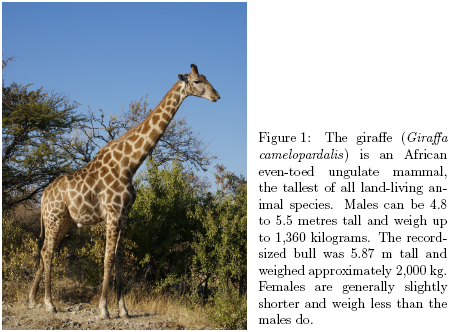
\includegraphics[width=0.48\textwidth]{./ingles/Latex_example_sidecap.jpg}
%  \end{center}
%\end{wrapfigure}

\begin{description}
\item[Nombre:] Martini Seco
\item[Cristaleria:] Copa Cóctel (4oz / 120cc)
\item[M\'etodo de elaboraci\'on:] Revuelto
\item[Decoraci\'on:] Aceituna
\end{description}

\begin{table}[h]
\caption{Ingredientes y proporciones} 
\label{tab:fonts}
\begin{center}       
\begin{tabular}{|l|l|l|c|l|} %% this creates two columns
%% |l|l| to left justify each column entry
%% |c|c| to center each column entry
%% use of \rule[]{}{} below opens up each row
\hline
\rule[-1ex]{0pt}{3.5ex}  \textbf{Producto} & \textbf{Bebida} & \textbf{Marca} & \textbf{Volumen} & \textbf{Fraccion}  \\
\hline
\rule[-1ex]{0pt}{3.5ex}  Aguardiente & Ginebra seca 			& Schlichte 		& 3 oz / 90 cc 	&  	\\
\hline
\rule[-1ex]{0pt}{3.5ex}  Vermouth 		& Cinzano Rosso 	& Cinzano 				& 1 oz / 30 cc 		&  	\\
\hline
\rule[-1ex]{0pt}{3.5ex}  Fruta 		& Limon & Gajo (s/ c\'ascara)	& 1		& 	\\
\hline
\rule[-1ex]{0pt}{3.5ex}  Fruta 		& Aceituna & Finca Cave Canem (s/ c\'ascara)	& 1		& 	\\
\hline
\end{tabular}
\end{center}
\end{table} 
\bigskip 

%%-----------------------------------------------------------
\subsubsection{Formato de elaboraci\'on} 
\label{sec:title}
\bigskip 
\begin{center}
\begin{enumerate}
\item Colocar en un vaso de composición 5 hielos, el vermouth, la ginebra y 10 gotas de lim\'on.
\item Revolver con la cucharilla mezcladora logrando que el l\'iquido se enfr\'ie.
\item Con un colador servir en la copa coctail, evitando servir el hielo.
\item Agregar una aceituna a la copa.

\end{enumerate}
\end{center}
\bigskip 
\bigskip 
%%%%%%%%%%%%%%%%%%%%%%%%%%%%%%%%%%%%%%%%%%%%%%%%%%%%%%%%%%%%%

\subsubsection{Notas}
\bigskip 
\begin{center}
\raggedright{}Servir sin sorbete.
\end{center} 

%\subsubsection{Informaci\'on extra}
\bigskip
%\begin{center}
\medskip 
%\raggedright{ \textbf{Or\'igenes de este trago}} \\ 
\medskip


%\end{center}